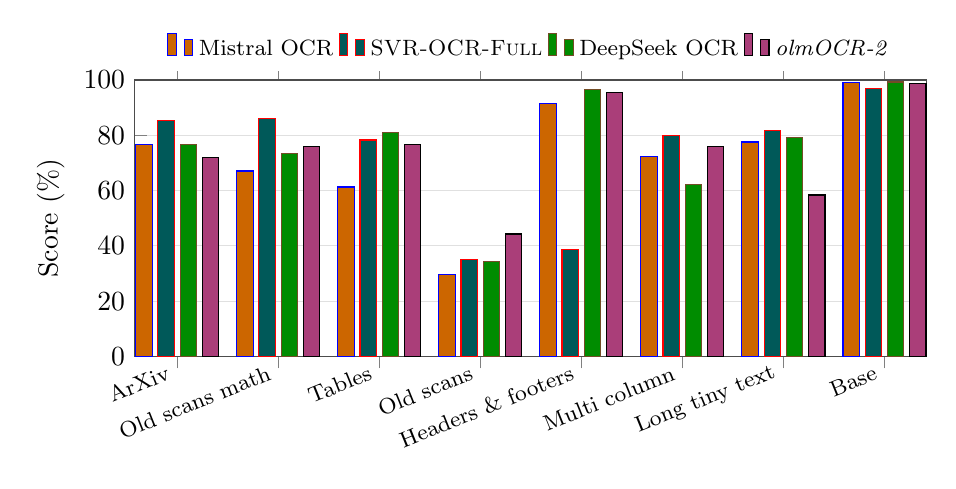
\begin{tikzpicture}
\begin{axis}[
    width=0.96\textwidth,
    height=0.42\textwidth,
    ybar,
    bar width=6pt,
    ymin=0,
    ymax=100,
    ylabel={Score (\%)},
    symbolic x coords={ArXiv,OldScansMath,Tables,OldScans,HeadersFooters,MultiColumn,LongTinyText,Base},
    xtick=data,
    xticklabels={ArXiv,Old scans math,Tables,Old scans,Headers \& footers,Multi column,Long tiny text,Base},
    x tick label style={font=\footnotesize, rotate=22, anchor=east},
    ytick={0,20,40,60,80,100},
    enlarge x limits=0.06,
    axis line style={black!70},
    ymajorgrids=true,
    grid style={draw=black!12},
    legend style={
        font=\footnotesize,
        draw=none,
        at={(0.5,1.03)},
        anchor=south,
        legend columns=4
    }
]
\addplot+[fill=orange!80!black] coordinates {
    (ArXiv,76.7)
    (OldScansMath,67.1)
    (Tables,61.3)
    (OldScans,29.8)
    (HeadersFooters,91.5)
    (MultiColumn,72.3)
    (LongTinyText,77.6)
    (Base,99.2)
};
\addplot+[fill=teal!70!black] coordinates {
    (ArXiv,85.3)
    (OldScansMath,86.0)
    (Tables,78.3)
    (OldScans,35.2)
    (HeadersFooters,38.8)
    (MultiColumn,79.8)
    (LongTinyText,81.7)
    (Base,97.1)
};
\addplot+[fill=green!55!black] coordinates {
    (ArXiv,76.6)
    (OldScansMath,73.5)
    (Tables,81.0)
    (OldScans,34.3)
    (HeadersFooters,96.6)
    (MultiColumn,62.2)
    (LongTinyText,79.1)
    (Base,99.3)
};
\addplot+[fill=magenta!65!black] coordinates {
    (ArXiv,71.9)
    (OldScansMath,76.0)
    (Tables,76.7)
    (OldScans,44.3)
    (HeadersFooters,95.4)
    (MultiColumn,76.1)
    (LongTinyText,58.4)
    (Base,98.8)
};
\legend{Mistral OCR,\textsc{SVR-OCR-Full},DeepSeek OCR,\textit{olmOCR-2}}
\end{axis}
\end{tikzpicture}
